% ------------------------------------------------------------------
% Chapter: Feature Selection (Phase 04)
% ------------------------------------------------------------------
\chapter{Feature Selection}
\label{chap:feature-selection}

\section{Ziel und Einordnung}
In dieser Phase wird die Eingangsmenge an Merkmalen für die Insolvenzprognose \emph{ökonometrisch} und \emph{validierungsstabil} reduziert. Die Auswahl dient drei Zielen: (i) Reduktion von Varianz und Komplexität, (ii) Vermeidung von Scheinkorrelationen und Datenleckage, (iii) Erhöhung der Interpretierbarkeit entlang betriebswirtschaftlicher Kategorien (Profitabilität, Liquidität, Leverage u.\,a.). Die Selektion erfolgt horizontspezifisch ($\mathrm{H1}$–$\mathrm{H5}$), da sich Informationshorizonte in ihren Signalträgern unterscheiden können. Die Entscheidung gegen rein \emph{black-box} getriebene Verfahren (z.\,B. tiefe neuronale Netze) erfolgt zugunsten prüffähiger, parsimoner Modelle mit expliziter Variablenlogik und belastbaren Stichprobenanforderungen (EPV) \parencite{rudin2019stop,wooldridge2010econometric}.

\section{Methodischer Rahmen und Gütekriterien}
Als prädiktive Gütekriterien werden ROC-AUC und PR-AUC verwendet; die PR-AUC ist bei Klassenungleichgewicht aussagekräftiger \parencite{saito2015precision}. Ergänzend wird die \emph{Stabilität der Auswahl} nach Nogueira berichtet \parencite{nogueira2018stability}, welche die Übereinstimmung der in den Validierungsfalten ausgewählten Merkmale quantifiziert. Ökonometrische Schutzschranken (``Guardrails'') steuern die Komplexität: Es gilt mindestens \emph{Events-per-Variable} $\mathrm{EPV}\geq10$ als konservative Daumenregel \parencite{peduzzi1996epv,steyerberg2019clinical}; zusätzlich wird gefordert, dass eine reduzierte Merkmalsmenge mindestens einen festgelegten Anteil der Baseline-Leistung beibehält.

\section{Vorgehensmodell}
Die Auswahl erfolgt methodenplural in drei Gruppen, um komplementäre Stärken auszunutzen und bekannte Verzerrungen einzelner Selektoren abzufedern \parencite{guyon2003introduction,meinshausen2010stability}.

\subsection{Filtermethoden}
Filtermethoden bewerten jedes Merkmal unabhängig vom Modell. Eingesetzt werden Spearman-Rangkorrelation (monotone Zusammenhänge), Mutual Information (nichtlineare Informationsgehalte) und ANOVA-F als parametrische Referenz. Da Finanzkennzahlen häufig nicht-normal und schief verteilt sind \parencite{mcleay2000prediction}, werden parametrische Annahmen (ANOVA-F) durch nichtparametrische bzw. informations-theoretische Größen (Spearman, MI) flankiert. Filter liefern robuste Grobvorschläge, sind jedoch blind für multivariate Substitutionseffekte.

\subsection{Wrappermethoden}
Wrapper (hier RFECV) nutzen ein Modell im Loop und entfernen Merkmale iterativ unter Kreuzvalidierung. Vorteile liegen in der Berücksichtigung von Interaktionen; Nachteile in Rechenaufwand und potenzieller Instabilität bei kleinen Effekten. Der Einsatz dient als Gegenpol zu rein univariaten Filtern \parencite{guyon2003introduction}.

\subsection{Eingebettete Methoden}
Eingebettete lineare Verfahren koppeln Auswahl und Schätzung: Lasso (L1), Elastic Net (L1/L2; \texttt{saga}) und Ridge (L2). Lasso fördert Sparsity, Elastic Net stabilisiert bei korrelierten Prädiktoren (Gruppenstruktur), Ridge liefert kontinuierliche Rangfolgen über Koeffizientenbeträge \parencite{hastieelementsstatistical2009}. Eine \emph{Pluralität} eingebetteter Verfahren erhöht die Chance, stabile \emph{Kerne} relevanter Merkmale zu identifizieren, wie auch Konzepte der Stability Selection nahelegen \parencite{meinshausen2010stability}. Als nichtlineare Referenz dient Random-Forest-Importance.

\section{Vom einfachen zum verschachtelten Ansatz}
Ein lediglich äußerer CV-Ansatz kann Auswahl-Bias erzeugen, wenn dieselben Daten die Merkmalsauswahl und die Leistungsbewertung speisen (Leckage). Um dies zu vermeiden, wird eine \emph{verschachtelte Kreuzvalidierung} verwendet: Pro äußerem Fold erfolgt die Merkmalsauswahl ausschließlich im Trainingssplit; die Bewertung wird auf dem zugehörigen Validierungssplit vorgenommen. Damit wird Auswahl-Bias reduziert und die Leistungsschätzung entkoppelt \parencite{cawley2010overfitting,varma2006bias}; zugleich wird Stabilität methodenübergreifend messbar.

\section{Stabilität der Auswahl}
Die Stabilität wird als korrigierte durchschnittliche Ähnlichkeit der foldweisen Auswahlen (nach Nogueira) definiert \parencite{nogueira2018stability}. Universelle Grenzwerte existieren nicht; empfohlen wird die \emph{relative} Interpretation im Methodenvergleich und über Horizonte hinweg. Werte näher an 1 deuten auf konsistentere Muster hin, Werte nahe 0 auf starke Variation.

\section{Konsensbildung unter Guardrails}
Aus den methodenspezifischen Auswahlen werden Konsensmengen konstruiert (Schnittmenge bzw. Mehrheitsregel). Anschließend werden Schutzschranken angewendet: (i) \textbf{EPV-Deckelung}: bei $E$ Ereignissen sind höchstens $\lfloor E/10 \rfloor$ Variablen zulässig; (ii) \textbf{Leistungs-Retention}: die reduzierte Menge muss mindestens einen festen Anteil der Baseline-ROC-AUC erreichen. Diese Schritte verhindern Überanpassung und sichern Interpretierbarkeit.

\section{Ergebnisse für H1 (verschachtelte Analyse)}
Für $\mathrm{H1}$ liegen verschachtelte Ergebnisse vor (5 Außenfalten; VIF-bereinigter Merkmalsraum gemäß Phase~03):
\begin{itemize}
	\item \textbf{Stabilität (Nogueira):} Ridge $0{,}454$, Lasso $0{,}327$, Elastic Net $0{,}050$. Im \emph{relativen} Vergleich zeigt Ridge konsistentere Auswahlmuster als Lasso/EN.
	\item \textbf{Fold-Mehrheit (\,$\geq 3/5$ Falten\,):} Lasso $n=36$, Elastic Net $n=40$, Ridge $n=28$. Größere Mehrheitsmengen bei Lasso/EN deuten auf geringere Übereinstimmung der Nullkoeffizienten.
	\item \textbf{Leistung (mittlere Außen-CV):} ROC-AUC Ridge $0{,}772$, Elastic Net $0{,}771$, Lasso $0{,}770$; PR-AUC ca. $0{,}138$–$0{,}140$. Die Unterschiede liegen im Bereich zufälliger Variation.
	\item \textbf{EPV-Implikation:} Bei gegebener Ereigniszahl $E$ sind maximal $\lfloor E/10 \rfloor$ Variablen zulässig \parencite{peduzzi1996epv,steyerberg2019clinical}. Mehrheitsmengen oberhalb dieser Schranke werden im Konsensschritt gekappt.
\end{itemize}
\noindent
\textit{Einordnung:} Die prädiktiven Leistungen unterscheiden sich für $\mathrm{H1}$ nur marginal; die PR-AUC bestätigt dies unter Klassenungleichgewicht \parencite{saito2015precision}. Stabilität wird \emph{relativ} interpretiert \parencite{nogueira2018stability}; im Vergleich weist Ridge robustere Muster auf. Für die Konsensbildung erhalten überlappende, stabile Merkmale größeres Gewicht; die EPV-Deckelung gewährleistet ökonometrische Vertretbarkeit. Damit liegen fokussierte, prüffähige Merkmalsmengen vor, die in Phase~05 als Eingangsgrößen für die Modellierung dienen, wo Generalisierung und Kalibrierung im Vordergrund stehen.

\subsection*{Hypothese vs. Beobachtung (H1)}
Als \emph{Hypothese} wurde anfänglich eine Rangfolge \enquote{Elastic Net $>$ Random Forest $>$ Lasso $>$ Ridge} diskutiert (Motivation: Gruppenstruktur korrelierter Kennzahlen). \emph{Beobachtung (nested)}: In $\mathrm{H1}$ liegen Lasso/Elastic Net/Ridge praktisch gleichauf (ROC-AUC $\approx 0{,}77$), mit einem leichten Vorteil für Ridge im alten Ansatz und einem konservativeren Wert unter Nested-CV. Die Unterschiede sind klein und im Bereich zufälliger Variation; maßgeblich für die Konsensbildung sind daher Stabilität und EPV-Vertretbarkeit.

\subsection*{Vergleich H1: Alter vs. verschachtelter Ansatz}
Zur Einordnung werden die Ergebnisse des ursprünglichen (nicht-verschachtelten) Ansatzes den verschachtelten Werten gegenübergestellt (alle Kennzahlen empirisch aus \\
\texttt{results/04\_feature\_selection/}):

\begin{table}[htbp]
\centering
\caption{Vergleich H1: Alter vs. verschachtelter Ansatz}
\label{tab:h1_comparison}
\begin{tabular}{lcccc}
\toprule
\textbf{Methode} & \textbf{ROC-AUC alt} & \textbf{ROC-AUC nested} & \textbf{PR-AUC alt} & \textbf{PR-AUC nested} \\
\midrule
Lasso & 0{,}7751 & 0{,}7700 & 0{,}1393 & 0{,}1375 \\
Elastic Net & 0{,}7707 & 0{,}7708 & 0{,}1390 & 0{,}1380 \\
Ridge & 0{,}7842 & 0{,}7724 & 0{,}1466 & 0{,}1396 \\
\bottomrule
\end{tabular}
\par\smallskip
{\footnotesize Quelle: Eigene Darstellung basierend auf Feature Selection Ergebnissen}
\end{table}

Der verschachtelte Ansatz liefert eine konservativere Leistungsschätzung (insb. Ridge, Konsistenz mit \parencite{cawley2010overfitting,varma2006bias}) und ermöglicht die Stabilitätsbewertung. Da die Leistungsdifferenzen insgesamt gering sind, wird zur Wahrung des Zeitbudgets die Modellierungsphase zunächst auf Basis der \emph{alten} H1–H5-Auswahlen durchgeführt; die verschachtelten Ergebnisse werden anschließend als Vergleich (Sensitivitätsanalyse) herangezogen.

\subsection*{Vergleich H2 und H3: Alter vs. verschachtelter Ansatz}
\paragraph{H2 (Embedded, linear):}
Alte (nicht-verschachtelte) vs. Nested-CV Ergebnisse (ROC-AUC):
\begin{itemize}
  \item Lasso: alt $0{,}7103$ \;$\rightarrow$\; nested $0{,}7085$ (\,$\Delta=-0{,}0018$\,)
  \item Elastic Net: alt $0{,}7086$ \;$\rightarrow$\; nested $0{,}7096$ (\,$\Delta=+0{,}0010$\,)
  \item Ridge: alt $0{,}7178$ \;$\rightarrow$\; nested $0{,}7082$ (\,$\Delta=-0{,}0096$\,)
\end{itemize}
Interpretation: Nested reduziert insbesondere bei Ridge den anfänglichen Optimismus. Insgesamt konvergieren die drei Verfahren bei $\approx 0{,}709$; kein klarer Sieger. Stabilität (Nogueira): Ridge $0{,}508$ $>$ Lasso $0{,}240$ $>$ Elastic Net $0{,}137$; für die Konsensbildung spricht dies für stärkere Gewichtung stabiler Kerne (Ridge/Lasso) und vorsichtige Nutzung breiter EN-Sets.

\paragraph{H3 (Embedded, linear):}
Alte (nicht-verschachtelte) vs. Nested-CV Ergebnisse (ROC-AUC):
\begin{itemize}
  \item Lasso: alt $0{,}7381$ \;$\rightarrow$\; nested $0{,}7339$ (\,$\Delta=-0{,}0042$\,)
  \item Elastic Net: alt $0{,}7416$ \;$\rightarrow$\; nested $0{,}7425$ (\,$\Delta=+0{,}0009$\,)
  \item Ridge: alt $0{,}7384$ \;$\rightarrow$\; nested $0{,}7347$ (\,$\Delta=-0{,}0037$\,)
\end{itemize}
Interpretation: Elastic Net bleibt knapp vorn, Unterschiede sind klein. Stabilität (Nogueira): Lasso $0{,}560$ $>$ Ridge $0{,}382$ $>$ Elastic Net $0{,}316$. Ergebnis: Je Horizont unterscheiden sich sowohl Rangfolge als auch Stabilität; daher ist ein konsensorientierter, EPV-gestützter Ansatz über Horizonte hinweg sachgerecht.

\paragraph{H4 (Embedded, linear; verschachtelt):}
Nested-CV (mittlere Außenfalten-ROC-AUC): Lasso $0{,}758$, Elastic Net $0{,}758$, Ridge $0{,}755$. Die Unterschiede sind klein; die \emph{Stabilität (Nogueira)} ist Ridge $0{,}455$ $>$ Elastic Net $0{,}312$ $>$ Lasso $0{,}199$ (H4). Damit bestätigt sich auch für H4: leichte Leistungsunterschiede, aber deutliche Stabilitätsunterschiede, was die Konsensorientierung stützt.

\section{Aggregierte Übersichten}
Die folgenden Tabellen fassen methodenspezifische Ergebnisse, Stabilitätskennzahlen und Konsensauswahlen zusammen. Die verschachtelten Stabilitätswerte werden fortlaufend ergänzt, sobald $\mathrm{H2}$–$\mathrm{H5}$ vorliegen.

\begin{figure}[H]
\centering
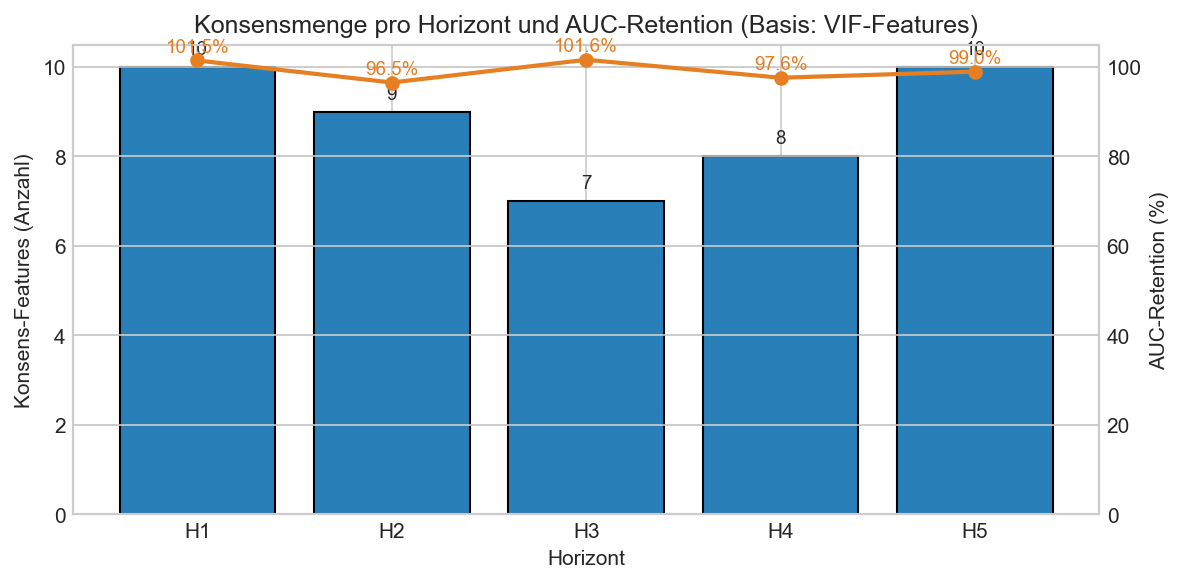
\includegraphics[width=0.9\textwidth]{figures/phase04/consensus_counts_retention.png}
\caption{Konsens-Featureanzahl und AUC-Retention je Horizont (Basis: VIF-Featuremenge)}
\label{fig:phase04_consensus_retention}
{\footnotesize Quelle: Eigene Darstellung basierend auf \texttt{04d\_ALL\_consensus.xlsx}}
\end{figure}

\subsection*{Methodenvergleich (ROC-AUC)}
\begin{table}[htbp]
\centering
\caption{Methodenvergleich (ROC-AUC)}
\label{tab:phase04_method_auc}
% Auto-generated: Phase 04 per-method ROC-AUC summary
% Columns: Horizon, Method, ROC-AUC (mean)
\begin{tabular}{l l r}
\toprule
Horizon & Method & ROC-AUC \\
\midrule
H1 & lasso & 0.770 \\
H1 & elastic\_net & 0.771 \\
H1 & ridge & 0.772 \\
H1 & random\_forest & 0.771 \\
H2 & lasso & 0.709 \\
H2 & elastic\_net & 0.710 \\
H2 & ridge & 0.708 \\
H2 & random\_forest & 0.709 \\
H3 & lasso & 0.734 \\
H3 & elastic\_net & 0.743 \\
H3 & ridge & 0.735 \\
H3 & random\_forest & 0.733 \\
H4 & lasso & 0.758 \\
H4 & elastic\_net & 0.758 \\
H4 & ridge & 0.755 \\
H4 & random\_forest & 0.747 \\
H5 & lasso & 0.854 \\
H5 & elastic\_net & 0.852 \\
H5 & ridge & 0.853 \\
H5 & random\_forest & 0.841 \\
\bottomrule
\end{tabular}

\par\smallskip
{\footnotesize Quelle: Eigene Darstellung basierend auf \texttt{results/04\_feature\_selection/}}
\end{table}

\subsection*{Stabilität über Falten (Nogueira)}
\begin{table}[htbp]
\centering
\caption{Stabilität über Falten (Nogueira)}
\label{tab:phase04_stability}
% Auto-generated: Phase 04 nested stability summary
% Columns: Horizon, Method, Stability
\begin{tabular}{l l r}
\toprule
Horizon & Method & Stability \\
\midrule
H1 & lasso & 0.327 \\
H1 & elastic\_net & 0.050 \\
H1 & ridge & 0.454 \\
H2 & lasso & 0.240 \\
H2 & elastic\_net & 0.137 \\
H2 & ridge & 0.508 \\
H3 & lasso & 0.560 \\
H3 & elastic\_net & 0.316 \\
H3 & ridge & 0.382 \\
H4 & lasso & 0.199 \\
H4 & elastic\_net & 0.312 \\
H4 & ridge & 0.455 \\
H5 & lasso & -- \\
H5 & elastic\_net & -- \\
H5 & ridge & -- \\
\bottomrule
\end{tabular}

\par\smallskip
{\footnotesize Quelle: Eigene Darstellung basierend auf \texttt{results/04\_feature\_selection/nested/}}
\end{table}

\subsection*{Konsens und Guardrails}
\begin{table}[htbp]
\centering
\caption{Konsens und Guardrails}
\label{tab:phase04_consensus}
% Auto-generated: Phase 04 consensus summary (intersection/majority)
% Columns: Horizon, Set, #Features, Retention
\begin{tabular}{l l r r}
\toprule
Horizon & Set & \#Features & Retention (\%) \\
\midrule
H1 & intersection & 10 & 101.5 \\
H2 & intersection & 9 & 96.5 \\
H3 & intersection & 7 & 101.6 \\
H4 & intersection & 8 & 97.6 \\
H5 & intersection & 10 & 99.0 \\
\bottomrule
\end{tabular}

\par\smallskip
{\footnotesize Quelle: Eigene Darstellung basierend auf \texttt{results/04\_feature\_selection/04d\_ALL\_consensus.xlsx}}
\end{table}

\section{Diagnostik und Robustheit}
Unter Klassenungleichgewicht können bei Elastic Net Konvergenzhinweise auftreten; dem wird durch adaptive Erhöhung von \texttt{max\_iter} und maßvolle Toleranzanpassung begegnet. Hyperparameter-Gitter werden so gesetzt, dass Rechenaufwand begrenzt und modelltheoretische Anforderungen (z.\,B. \texttt{saga} für Elastic Net) erfüllt werden \parencite{hastieelementsstatistical2009}. Die Stabilitätsanalyse ergänzt die prädiktive Leistung als zweite Robustheitsachse.

\textbf{Validierung theoriebasierter Entscheidungen:} Die Feature Selection bestätigt exemplarisch die Robustheit der Pipeline. So wurde beispielsweise Kennzahl A37 (\textit{Quick Assets / Long-term Liabilities}) trotz problematischer Imputationsqualität (43,7\,\% fehlende Werte, Quality Score 25/100) in der Datenaufbereitung (Abschnitt 4.3) zunächst aus theoretischen Gründen beibehalten. Die datengetriebene Feature Selection eliminierte A37 jedoch über alle Horizonte hinweg aus den finalen Konsensmengen – eine Bestätigung, dass die Pipeline problematische Features algorithmisch identifiziert und entfernt, selbst wenn sie theoretisch plausibel erscheinen.

Die resultierenden, EPV-konformen Konsensmengen schließen nahtlos an Phase~05 an, in der diese Merkmalsmengen in logistischen Modellen und Waldverfahren als finale Inputs dienen und gegen Baselines gespiegelt werden.
